\section{Theory}
\vspace{-0.5cm}
\singlespacing

Acceleration due to gravity only impacts the vertical component of motion. This means that a projectile shot horizontally and one dropped a the same height, will have the same amount of time in the air. \par

\begin{figure}[H]
	\begin{center}
		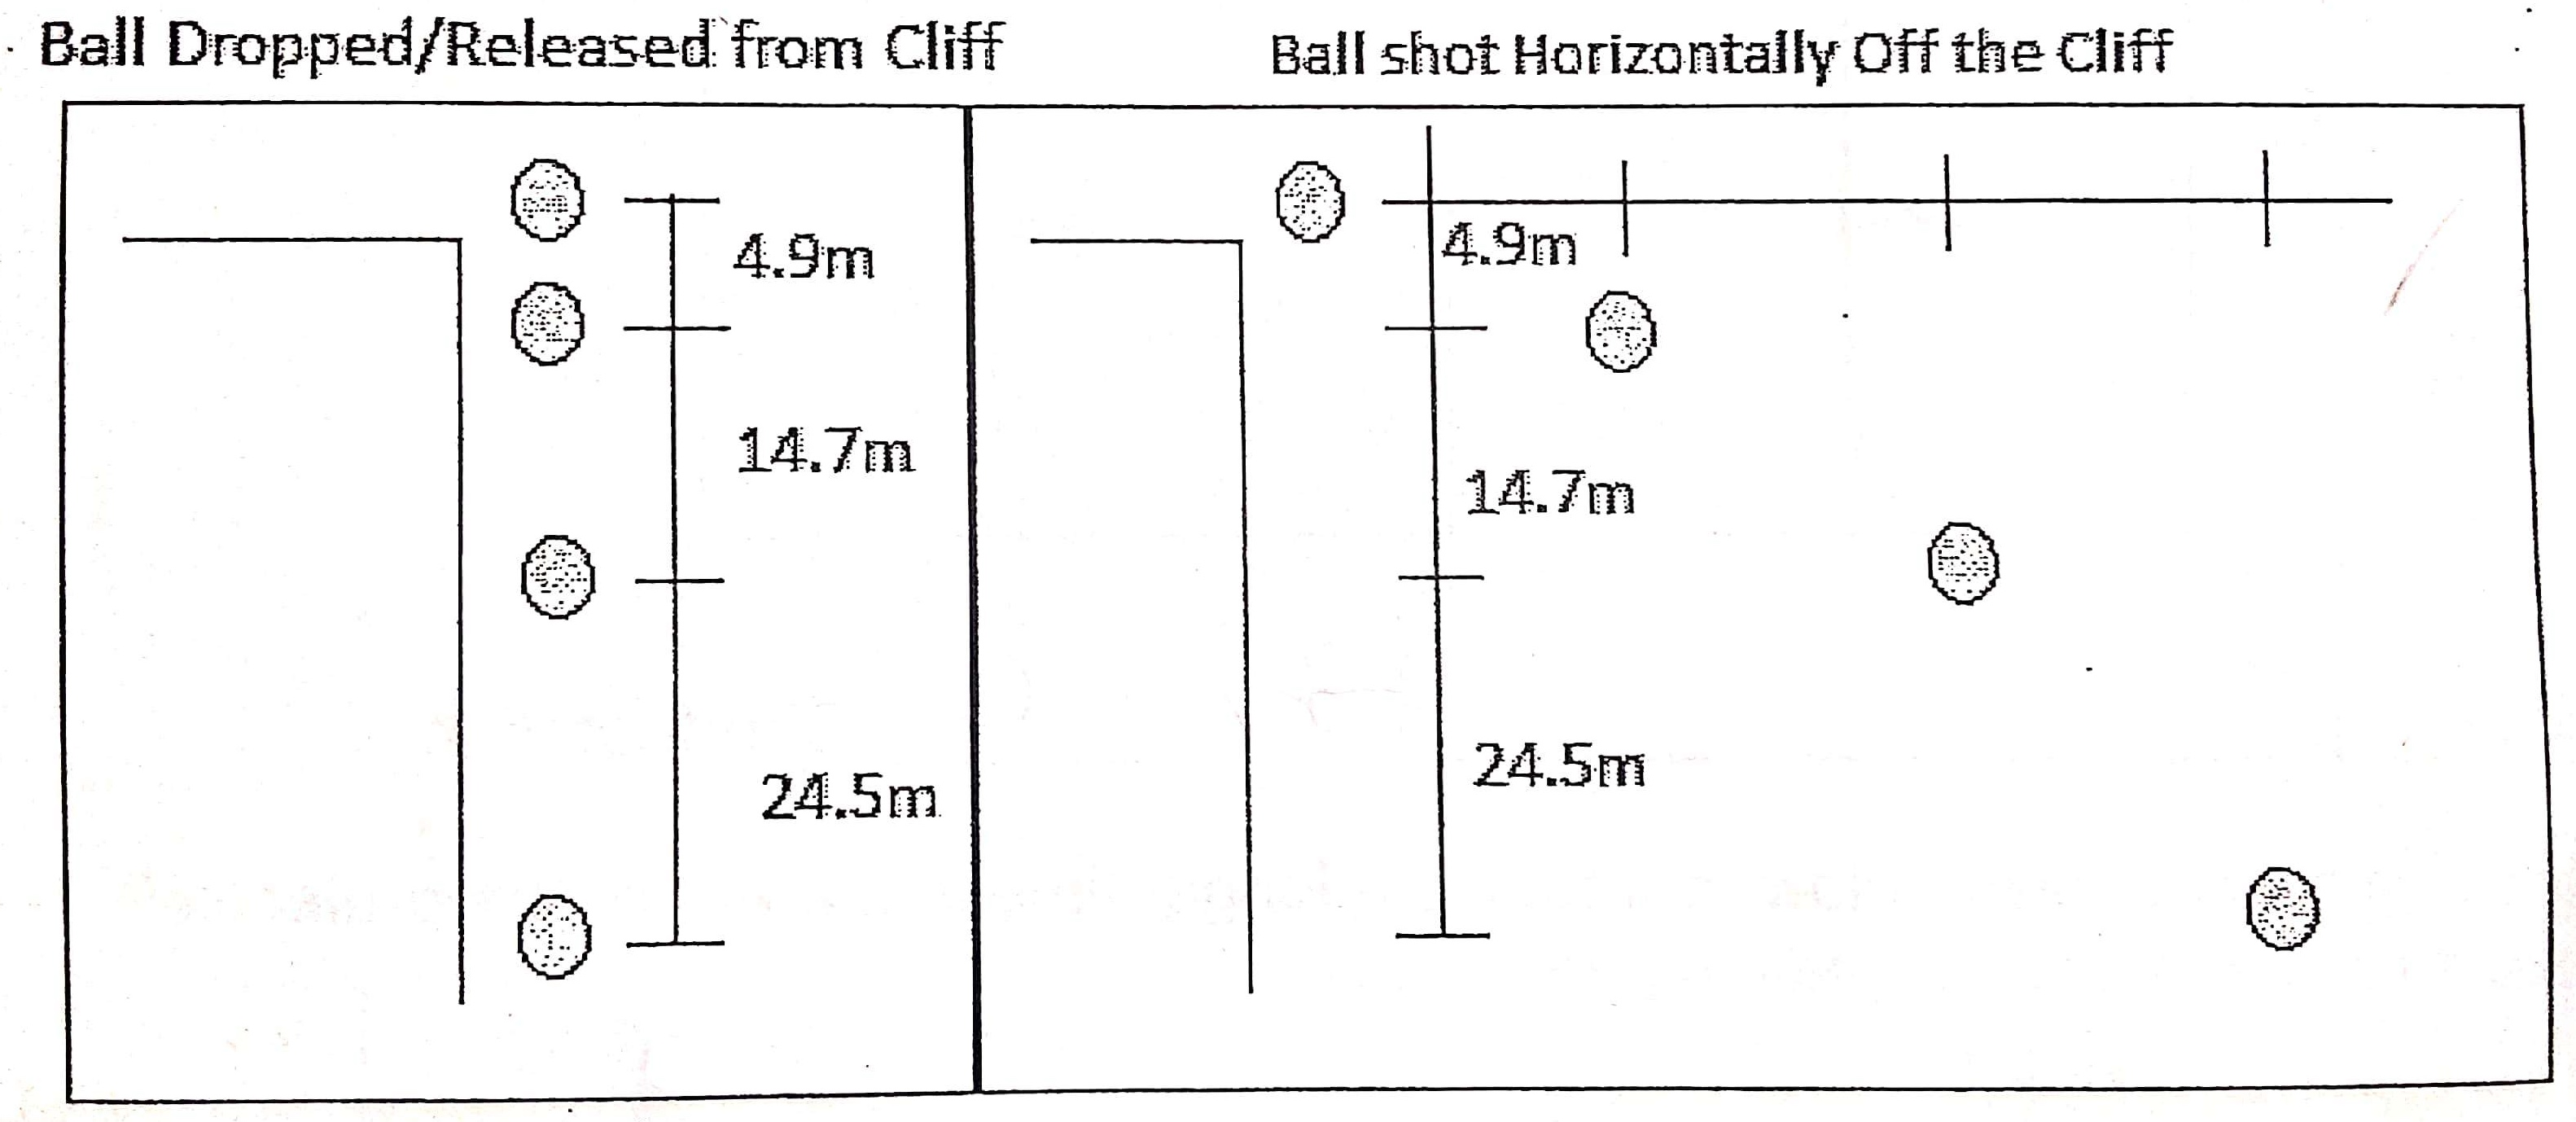
\includegraphics[width=0.75\textwidth]{images/2DMotion}
	\end{center}
	\caption{A ball dropped from a height will hit the ground at the same time as a ball
 that is launched horizontally, since gravity only impacts the vertical component of motion.}\label{fig:2DMotion}
\end{figure}

Since gravity only affects the vertical component of motion, then, assuming no air resistance, the initial horizontal velocity of an object will be the same throughout its motion. More specifically, the acceleration due to gravity of an object in the horizontal direction is $0\,m/s^2$, while in the vertical direction its $-9.8\,m/s^2$. This difference in accelerations in the x and y directions slightly changes the equations of kinematics used. All the equations of kinematics used for 1D motion still apply in the y direction, however, since acceleration due to gravity in the x direction is $0\,m/s^2$, the horizontal distance an object travels can be easily determined using the following equation:

\vspace{-0.5cm}
\begin{equation*}
	x = V\!o_xt
\end{equation*}

When dealing with objects fired at angles, we must use trigonometric functions to seperate the x and y directions (the same way one would break up a vector into x and y components). The following equations can be used to determine the initial velocity of an object in the x and y directions:

\begin{equation*}
\begin{aligned}
	V\!o_x = V\!osin(\theta) \\
	V\!o_y = V\!ocos(\theta)
\end{aligned}
\end{equation*}
\newpage

